\documentclass[conference]{IEEEtran}
\usepackage{cite}
\usepackage[pdftex]{graphicx}
\usepackage{amsmath}
\usepackage{booktabs}
\usepackage{xcolor}
\usepackage{listings}
\lstset{basicstyle=\ttfamily,
	showstringspaces=false,
	commentstyle=\color{red},
	keywordstyle=\color{blue}
}


\begin{document}
\title{Practical Assignment\\ {\fontsize{13}{0}\selectfont 2IMN15: Internet of Things } \\ {\fontsize{13}{0}\selectfont \today }\\{ \fontsize{13}{0}\selectfont Group 14: Broker Team - Blue}}

\author{\IEEEauthorblockN{Sai Krishna Kalluri}
	\IEEEauthorblockA{TU/e, Netherlands\\
		Email: saikrishh.kalluri@gmail.com}
	\and
	\IEEEauthorblockN{Snorri Stefansson}
	\IEEEauthorblockA{TU/e, Netherlands\\
		Email: snorriste@gmail.com}}
\maketitle

\IEEEpeerreviewmaketitle


\begin{abstract}
	This practical assignment for the course IoT involves creating a lightning system controlled and managed by different but relevant wireless protocols and separated individual applications. The architecture and development of this system will be the topic of this report.\\
	
\end{abstract}


\section{Introduction}

The goal is to 



\section{Architecture and Protocols}

\begin{figure}[h]
	\begin{center}
		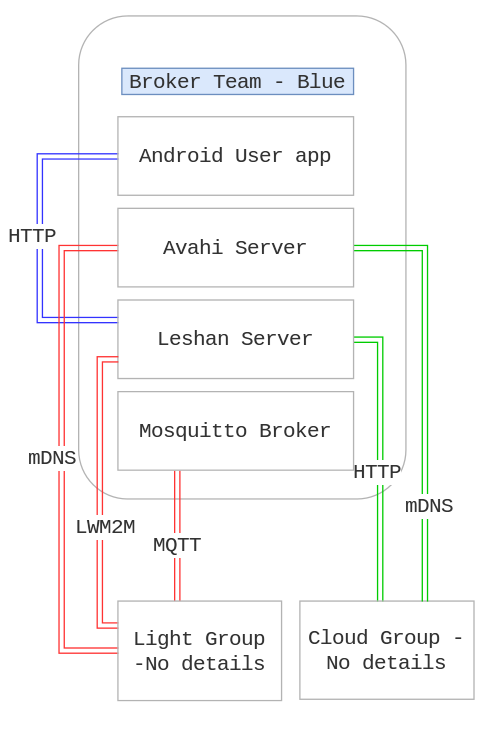
\includegraphics[width=1\linewidth]{img/overview}
		\caption{}
		\label{fig:fig1}
	\end{center}
\end{figure}
\subsection{LWM2M, CoAP and HTTP with Leshan}
Leshan infrastructure, protocols used and relevance to project

\subsection{mDNS with Avahi server}
\subsection{MQTT with Mosquitto}
\subsection{User app - Android}

\begin{figure}[h]
	\begin{center}
		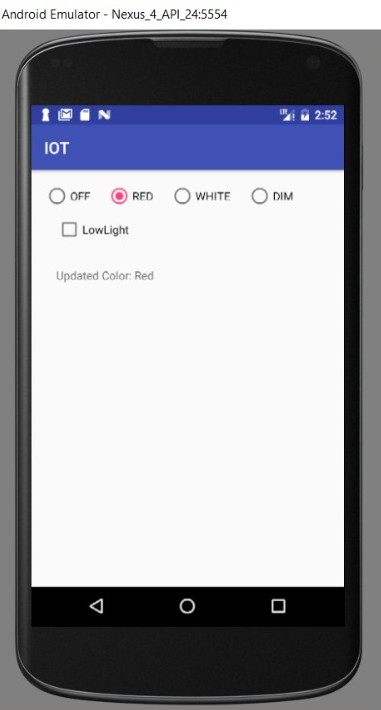
\includegraphics[width=1\linewidth]{img/androidapp}
		\caption{}
		\label{fig:fig2}
	\end{center}
\end{figure}


\section{Operations}

\subsection{Initialization}

\subsection{Use cases - post init}

\section{Discussion and results}

\section{Conclusion}






\begin{lstlisting}[basicstyle=\tiny,language=python,caption={Code}]

Code snippet
\end{lstlisting}

\end{document}